\newcommand{\demorows}{10175}
\newcommand{\labexrows}{9813}

\section{Experiments}\label{sec:experiments}
To evaluate the performance of our approach,  we implemented
a prototype system in Java, following a traditional iterator model.
For our experiments we plan and execute queries
for two separate survey-based data sets, showing that our system
is well suited for early dataset exploration.

\subsection{Data sets} \label{subsec:datasets}
We collected three data sets our experiments.
For all data sets, we selected a subset of the original attributes.
We also enumerated strings and encoded them with an appropriate integer value.
\todo{describe all data transformations. jose?}

\subsubsection{CDC NHANES}
For our first set of experiments, we use survey data collected by the 
Centers for Disease Control and Prevention (CDC) in the United States. We
experiment on a set of tables collected as part of the 2013--2014 National
Health and Nutrition Examination Survey (NHANES), a series of studies
conducted by the CDC on a national sample of several thousand individuals~\cite{cdc-data}.
The data consists on survey responses, physical examinations, and laboratory
results, amongst others.

There are 6 tables in the NHANES data set. We use three tables for our experiments:

\begin{itemize}
	\item \emph{Demographics}: demographic information of subjects
	\item \emph{Examinations}: physical exam results
	\item \emph{Laboratory}: laboratory exam results
\end{itemize}

The original tables have a large number of attributes, in some cases providing more granular tests results or alternative metrics.
We focused on a subset of the attributes for each table to simplify the presentation and exploration of queries.
\Cref{table:nhanes-description} shows the attributes selected, along with the percentage of null values for each attribute.
For readability, we have replaced the NHANES variable names with self-explanatory attribute names.

\begin{table}
  \centering
  \begin{subtable}{0.5\textwidth}
    \centering
    \begin{tabular}{llr}
\toprule
\textbf{Attribute} &  \textbf{\% Missing} \\
\midrule
age\_months &      93.39 \\
age\_yrs &       0.00 \\
gender &       0.00 \\
id &       0.00 \\
income &       1.31 \\
is\_citizen &       0.04 \\
marital\_status &      43.30 \\
num\_people\_household &       0.00 \\
time\_in\_us &      81.25 \\
years\_edu\_children &      72.45 \\
\bottomrule
\end{tabular}

    \caption{Demographics. \demorows{} rows.}
  \end{subtable}
  \par\medskip
  \begin{subtable}{0.5\textwidth}
    \centering
    \begin{tabular}{lS[table-format=2.2]}
\toprule
\textbf{Attribute} &  \textbf{Missing} \\
\midrule
albumin &      17.95\ \% \\
blood\_lead &      46.86\ \% \\
blood\_selenium &      46.86\ \% \\
cholesterol &      22.31\ \% \\
creatine &      72.59\ \% \\
hematocrit &      12.93\ \% \\
id &       0.00\ \% \\
triglyceride &      67.94\ \% \\
vitamin\_b12 &      45.83\ \% \\
white\_blood\_cell\_ct &      12.93\ \% \\
\bottomrule
\end{tabular}

%%% Local Variables:
%%% mode: latex
%%% TeX-master: "../main"
%%% End:

    \caption{Laboratory Results. \labexrows{} rows.}
  \end{subtable}
  \par\medskip  
  \begin{subtable}{0.5\textwidth}
    \centering
    \begin{tabular}{llr}
\toprule
 Table &                Attribute &  \% Missing \\
\midrule
 exams &        arm\_circumference &       5.22 \\
 exams &      blood\_pressure\_secs &       3.11 \\
 exams &  blood\_pressure\_systolic &      26.91 \\
 exams &          body\_mass\_index &       7.72 \\
 exams &                cuff\_size &      23.14 \\
 exams &       head\_circumference &      97.67 \\
 exams &                   height &       7.60 \\
 exams &                       id &       0.00 \\
 exams &      waist\_circumference &      11.74 \\
 exams &                   weight &       0.92 \\
\bottomrule
\end{tabular}

    \caption{Physical Results. \labexrows{} rows.}
  \end{subtable}
  \par\medskip  
  \caption{Missing value distribution for each table/attribute in CDC NHANES 2013--2014 data.}\label{table:nhanes-description} 
\end{table}

\subsubsection{freeCodeCamp 2016 New Coder Survey}
For our second set of experiments, we chose to use data collected
by freeCodeCamp (FCC) as a part of a survey of new software developers
(both professional and amateur)~\cite{fcc-data}. freeCodeCamp is an open-source
community that helps users learn how to program. Their \textit{2016 New Coder Survey} consists of responses by over 15,000 people to 48 different
demographic and programming-related questions.
The survey targeted users who were related to coding organizations.

We use a version of the data that has been pre-processed, but where missing values remain.
\todobox{Give example of expected missing value}{However, many of the missing values are expected because the data has been de-normalized.}
The original dataset has 15,620 rows and 113 attributes.
We chose a subset of 17 attributes, shown in~\Cref{table:fcc-description}, along with the percentage of missing values.

\begin{table}
  \centering
  \begin{tabular}{lr}
\toprule
            \textbf{Attribute} &  \textbf{\% Missing} \\
\midrule
age &      12.85 \\
attendedbootcamp &       1.54 \\
 bootcampfinish &      94.03 \\
 bootcampfulljobafter &      95.93 \\
 bootcamploanyesno &      94.02 \\
 bootcamppostsalary &      97.89 \\
childrennumber &      83.65 \\
citypopulation &      12.74 \\
commutetime &      46.61 \\
countrycitizen &      12.59 \\
gender &      12.00 \\
hourslearning &       4.34 \\
income &      53.08 \\
moneyforlearning &       6.02 \\
monthsprogramming &       3.88 \\
schooldegree &      12.43 \\
studentdebtowe &      77.50 \\
\bottomrule
\end{tabular}

  \caption{Missing values in freeCodeCamp Survey Data}\label{table:fcc-description} 
\end{table}

\subsubsection{American Community Survey}
For our final experiment, we introduce a simple aggregate query over data from the American Community Survey (ACS), which
provides a number of public data sets collected by the U.S. Census Bureau.
We used a cleaned version of the 2012 Public Use Microdata Sample (PUMS) data kindly provided by the authors of~\cite{akande2015empirical}.
Given that the data had been cleaned, we artificially dirtied it by removing 40\% of the values uniformly at random.
The final dataset consists of 671,153 rows and 37 integer columns.

\subsection{Queries}
We collected a set of queries (\Cref{fig:queries}) that we think are interesting to plan.
We believe that they could reasonably be written by a user in the course of data analysis.

The queries on the CDC NHANES data consist not only of projections and selections, but also interesting joins and aggregates.
Our aim was to craft meaningful queries
that would provide performance figures relevant to practitioners using
similar datasets.

Our first set of queries is on the CDC data (\Cref{fig:queries-cdc}). In~\Cref{q1}, we
calculate the average height for users based on their income data. In~\Cref{q2}, we compare
cholesterol levels for individuals with low, medium, and high incomes spectrum and above a
certain weight. In~\Cref{q3}, we extract the maximum blood lead levels for children under
the age of 6 years. In~\Cref{q4}, we calculate the average systolic blood pressure, by
gender, for subjects with a body mass index indicating obesity. 

Our second set of queries is on the FCC data (\Cref{fig:queries-fcc}).
\Cref{q5} calculates the average income for survey participants, based on their bootcamp attendance.
\Cref{q6} estimates the average age of women from the United States who participated.
\Cref{q7} calculates the average amount of money survey participants with student debt spent on learning based on their school degree.
\Cref{q8} joins the freeCodeCamp data with a reference table provided by the World Bank which summarizes GDP per-capita across various countries~\cite{worldbank-data}.
The query calculates the average GDP per-capita of countries with and without bootcamp participants. 
\begin{table*}
\centering
 \begin{subtable}{\linewidth}
  \newcounter{queryno}
\begin{tabular}{cl}
\toprule
\# & \multicolumn{1}{c}{Query} \\
\midrule
1 & 
\begin{minipage}{6in}
\begin{lstlisting}[breaklines]
SELECT income, AVG(height)
FROM demo, exams
WHERE demo.id = exams.id
GROUP BY income;
\end{lstlisting}
\end{minipage}\refstepcounter{queryno} \label{q1} \\
2 & 
\begin{minipage}{6in}
\begin{lstlisting}[breaklines]
SELECT income, AVG(cholesterol)
FROM demo, exams, labs
WHERE demo.id = exams.id AND exams.id = labs.id AND
      income >= 13 AND income <= 15 AND weight >= 63
GROUP BY income;
\end{lstlisting}
\end{minipage}
\refstepcounter{queryno} \label{q2} \\
3 & 
\begin{minipage}{6in}
\begin{lstlisting}[breaklines]
SELECT MAX(blood_lead)
FROM demo, exams, labs
WHERE demo.id = labs.id AND labs.id = exams.id AND age_yrs <= 6;
\end{lstlisting}
\end{minipage}\refstepcounter{queryno} \label{q3}\\
4 & 
\begin{minipage}{6in}
\begin{lstlisting}[breaklines]
SELECT gender, AVG(blood_pressure_systolic)
FROM demo, labs, exams
WHERE demo.id = labs.id AND labs.id = exams.id AND
      body_mass_index >= 30
GROUP BY gender;
\end{lstlisting}
\end{minipage}\refstepcounter{queryno} \label{q4}\\
%5 & 
%\begin{minipage}{6in}
%\begin{lstlisting}[breaklines]
%SELECT age_yrs, gender, triglyceride, waist_circumference
%FROM demo, labs, exams
%WHERE demo.id = exams.id AND labs.id = exams.id AND
%      labs.triglyceride > 200;
%\end{lstlisting}
%\end{minipage}\refstepcounter{queryno} \label{q5}\\
\bottomrule
\end{tabular}

  \caption{Queries on CDC data}
  \label{fig:queries-cdc}
 \end{subtable}
 ~
 \begin{subtable}{\linewidth}
 \begin{tabular}{cl}
\toprule
\# & \multicolumn{1}{c}{Query} \\
\midrule
6 & 
\begin{minipage}{6in}
\begin{lstlisting}[breaklines]
SELECT attendedbootcamp, AVG(income)
FROM fcc
GROUP BY attendedbootcamp;
\end{lstlisting}
\end{minipage}\refstepcounter{queryno} \label{q6} \\
7 & 
\begin{minipage}{6in}
\begin{lstlisting}[breaklines]
SELECT AVG(age)
FROM fcc
WHERE gender = 178 AND countrycitizen = 158;
\end{lstlisting}
\end{minipage}\refstepcounter{queryno} \label{q7} \\
8 & 
\begin{minipage}{6in}
\begin{lstlisting}[breaklines]
SELECT schooldegree, AVG(moneyforlearning)
FROM fcc
WHERE studentdebtowe > 0 AND schooldegree >= 0
GROUP BY schooldegree;
\end{lstlisting}
\end{minipage}\refstepcounter{queryno} \label{q8}\\
9 & 
\begin{minipage}{6in}
\begin{lstlisting}[breaklines]
SELECT attendedbootcamp, AVG(gdp_per_capita)
FROM fcc, gdp
WHERE fcc.countrycitizen = gdp.country
GROUP BY attendedbootcamp;
\end{lstlisting}
\end{minipage}\refstepcounter{queryno} \label{q9}\\
10 & 
\begin{minipage}{6in}
\begin{lstlisting}[breaklines]
SELECT bootcamppostsalary, gdp_per_capita
FROM fcc, gdp
WHERE fcc.countrycitizen = gdp.country AND
      fcc.bootcamppostsalary <= 2 AND
      gdp.gdp_per_capita <= 5000;
\end{lstlisting}
\end{minipage}\refstepcounter{queryno} \label{q10}\\
\bottomrule
\end{tabular}

 \caption{Queries on FCC data}
 \label{fig:queries-fcc}
 \end{subtable}
 ~
 \begin{subtable}{\linewidth}
 \begin{tabular}{cl}
\toprule
\# & \multicolumn{1}{c}{Query} \\
\midrule
9 & 
\begin{minipage}{6in}
\begin{lstlisting}[breaklines]
SELECT AVG(c0) FROM acs_dirty;
\end{lstlisting}
\end{minipage}\refstepcounter{queryno} \label[query]{q9} \\
\bottomrule
\end{tabular}

 \caption{Queries on ACS data}
 \label{fig:query-acs}
 \end{subtable}

  \caption{Queries used in our experiments.}
  \label{fig:queries}
\end{table*}

%\begin{table*}
%  \centerfloat
%  \begin{tabular}{cSSSSSSS}
\toprule
\multicolumn{2}{c}{} & \multicolumn{2}{c}{Imputed ($\alpha=0.0$)} & \multicolumn{2}{c}{Imputed ($\alpha=1.0$)} \\
\cmidrule(r){3-4}
\cmidrule(l){5-6}
\# & \multicolumn{1}{c}{Base error} & \multicolumn{1}{c}{Error} & \multicolumn{1}{c}{Time (s)} & \multicolumn{1}{c}{Error} & \multicolumn{1}{c}{Time (s)} \\
\midrule
\ref{q1} & 5.25e+03 & 0.00e+00 & 1.723 & -3.60e+03 & 11.008 \\
\ref{q2} & 3.38e+04 & 0.00e+00 & 1.748 & -3.37e+04 & 10.144 \\
\ref{q3} & 9.32e-04 & 0.00e+00 & 1.732 & 2.54e-02 & 33.04 \\
\ref{q4} & 1.78e+05 & 0.00e+00 & 1.778 & -1.55e+05 & 21.013 \\
\ref{q5} & 9.89e-04 & 0.00e+00 & 1.712 & 9.89e-02 & 7.981 \\
\ref{q6} & 1.01e-02 & 0.00e+00 & 1.982 & 1.13e-02 & 52.309 \\
\ref{q7} & 0.00e+00 & 0.00e+00 & 43M49.786 & 0.00e+00 & 5.946 \\
\ref{q8} & 0.00e+00 & 0.00e+00 & 1.776 & 0.00e+00 & 3.172 \\
\ref{q9} & \multicolumn{1}{c}{--} & \multicolumn{1}{c}{--} & 1.919 & \multicolumn{1}{c}{--} & 2M40.384 \\
\ref{q10} & \multicolumn{1}{c}{--} & \multicolumn{1}{c}{--} & 0.01 & \multicolumn{1}{c}{--} & 7.786 \\
\ref{q11} & \multicolumn{1}{c}{--} & \multicolumn{1}{c}{--} & 0.007 & \multicolumn{1}{c}{--} & 0.103 \\
\ref{q12} & 0.00e+00 & 0.00e+00 & 0.008 & 1.00e-02 & 0.175 \\
\ref{q13} & \multicolumn{1}{c}{--} & \multicolumn{1}{c}{--} & 0.407 & \multicolumn{1}{c}{--} & 0.4 \\
\ref{q14} & 0.00e+00 & 0.00e+00 & 0.752 & 4.37e-01 & 1M14.221 \\
\bottomrule
\end{tabular}

%    \caption{Base error, percent change in error and and running time for queries
%    with different imputation levels. Base error is the root-mean-square error (RMSE) between the query run on clean
%    data and the query run on dirty data without imputation. Change in error is relative to the base error.}
%  \label{fig:experiments}
%\end{table*}

All experiments were run on a single Amazon Web Services EC2 {\tt c4.xlarge} instance, with
four 2.9 GHz Intel Xeon E5--2666 v3 virtual CPUs and 7.5 GiB of main memory, on Debian Linux.

\Cref{fig:runtimes} shows a summary of the performance results. The first plot
shows average running times for \ProjectName{} plans in two configurations:
quality-optimized and runtime-optimized. The second plot shows, for comparison, the average
running times required for each query when performing imputation at the base tables.  In all
cases, running a query through \ProjectName{} is cheaper than imputing a single base table,
with performance improvement on a factor of ten\todo{give range of performance}. This performance differential means it is feasible
to explore multiple imputations operations (including more expensive operators) when using
\ProjectName{}, in contrast to the traditional approach of base table imputation.

\begin{figure}
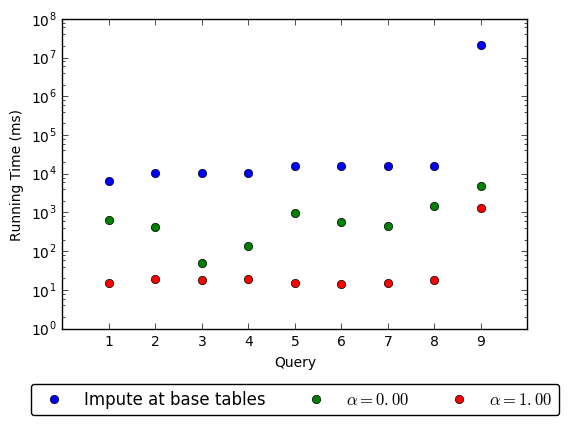
\includegraphics[width=\columnwidth]{figures/running_times_combined.png}
\caption{Query runtimes with imputation on base tables, \ProjectName{} imputation
    optimizing for quality ($\alpha=0$), and \ProjectName{} imputation optimizing for
    efficiency ($\alpha=1$). Quality-optimized, on-the-fly imputation provides an order of
    magnitude speedup over imputing on base tables. Efficiency-optimized on-the-fly
    imputation can provide another order-of-magnitude speedup at the expense of quality. For
    relatively large queries (Query 9), runtime of imputation can be reduced from 6.5
    hours to 7 seconds. }
\label{fig:runtimes}
\end{figure}

%\Cref{fig:plantimes} provides a summary of the planning times for each of the queries.
%We exclude the planning time for queries that impute at base table, as that requires no
%planning. 

In the median query across a variety of queries and choices of $\alpha$, planning
constituted 8.5 percent of total runtime. In all cases, the optimizer
returned a query plan within 40ms, with times roughly constant between levels of $\alpha$.

% The one-standard-deviation
%intervals around the mean planning time often overlap, suggesting the planning component is
%constant in $\alpha$.

%\begin{figure}
%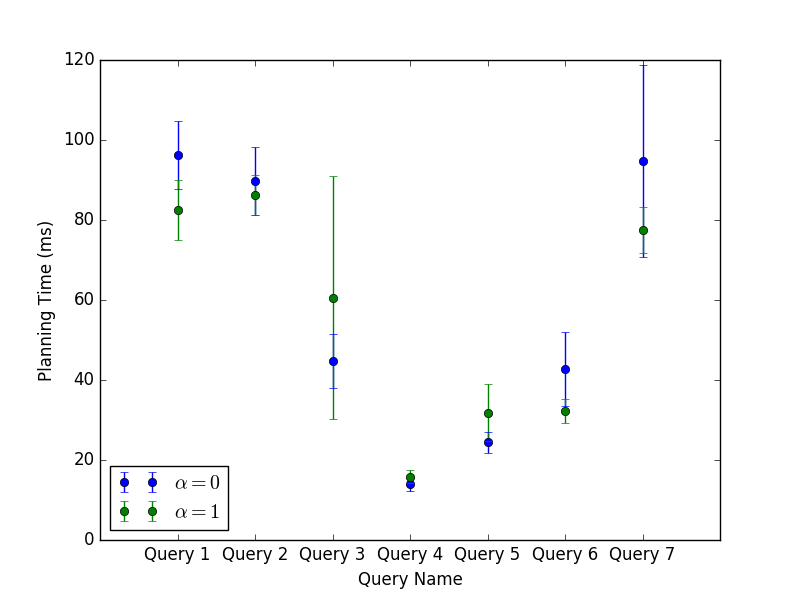
\includegraphics[width=\columnwidth]{figures/planning_times_imputedb.png}
%\caption{Planning times for each query}
%\label{fig:plantimes}
%\end{figure}

\Cref{table:smape} shows the Symmetric-Mean-Absolute-Percentage-Error (SMAPE) for \ProjectName{}'s query results when compared to running imputation on the base tables and executing the query on the cleaned data \todo{SMAPE citation}.
Each query was separately run 200 times in both settings and then results from the two approaches were paired up and compared tuple-wise.
We average tuple-wise absolute percentage deviations within each iteration of a query, and we report this value averaged over all iterations.
We can see that optimizing for quality indeed reduces the SMAPE of query results.
In general, the SMAPE relative to the base-imputation approach are low in all cases\todo{give actual value}, indicating that on-the-fly imputation produces similar results to imputation at the base tables.

\begin{table}
\todo{Consider switching to graph, or changing table layout..not very intuitive right now.}
\centering
\begin{tabular}{rrr}
\toprule
 Query &  \textbackslashalpha &  SMAPE \\
\midrule
     0 &     0.0 &   0.47 \\
     0 &     1.0 &   0.15 \\
     1 &     0.0 &   0.28 \\
     1 &     1.0 &   0.40 \\
     2 &     0.0 &   0.00 \\
     2 &     1.0 &   0.00 \\
     3 &     0.0 &   0.03 \\
     3 &     1.0 &   0.22 \\
     4 &     0.0 &  11.18 \\
     4 &     1.0 &    NaN \\
     5 &     0.0 &   0.79 \\
     5 &     1.0 &   1.93 \\
     6 &     0.0 &   0.00 \\
     6 &     1.0 &   0.03 \\
     7 &     0.0 &   0.82 \\
     7 &     1.0 &  35.44 \\
     8 &     0.0 &   0.23 \\
     8 &     1.0 &   0.31 \\
     9 &     0.0 & 100.00 \\
     9 &     1.0 & 100.00 \\
\bottomrule
\end{tabular}

\caption{Symmetric-Mean-Absolute-Percentage-Error for queries run under different $\alpha$
    parameterizations relative to results when imputing on base table. Values of $0.0$,
    $100.0$, or $NaN$ indicate uninformative values\todo{use one flag value (-) or explain why value is uninformative}.} %TODO MJS
\label{table:smape}
\end{table}

In many real-world cases, applying the imputation step at the base table is prohibitively
expensive.
To illustrate the increasing difficulty of such an approach as datasets scale, we run the
query in (\Cref{fig:query-acs}) over the ACS dataset.
Applying the imputation operation to the base table is extremely expensive, in our case
completing in 355 minutes(\ref{fig:runtimes}). In contrast, \ProjectName{} executes a quality-optimized version
in 7 seconds and a runtime-optimized version in 1 second. This highlights the potential
benefit of using our system for early data exploration.

%%% Local Variables:
%%% mode: latex
%%% TeX-master: "main"
%%% End:
